\chapter{معماری فنی و پروتکل‌های \lr{QKD}}
\label{chap:qkdarchitecture}
%=====================================================================

\section{دسته‌بندی پروتکل‌ها}

پروتکل‌های \lr{QKD} تجاری امروزی را می‌توان در سه خانوادهٔ اصلی دسته‌بندی کرد که در جدول \ref{tab:protocols} خلاصه شده‌اند.

\begin{table}[htbp]
\centering
\caption{مقایسهٔ خانواده‌های اصلی پروتکل‌های \lr{QKD} تجاری \Cite{arxiv2507maturity}}
\label{tab:protocols}
\small
\begin{tabular}{p{2.6cm}p{4.3cm}p{3.5cm}p{3.5cm}}
\toprule
\textbf{خانواده} & \textbf{توضیح فنی} & \textbf{برد معمول} & \textbf{تولیدکنندگان نمونه} \\
\midrule
\lr{DV-QKD} (متغیر گسسته) & کدگذاری بر پایهٔ فوتون‌های تکی و آشکارسازهای تک‌فوتونی؛ شامل \lr{BB84}، \lr{decoy-state}، \lr{COW} & تا $\sim 200$ کیلومتر (بدون گره میانی) & \lr{ID Quantique}، \lr{Toshiba} \\
\lr{CV-QKD} (متغیر پیوسته) & استفاده از آشکارسازی همدوس \lr{(Coherent Detection)} مشابه مخابرات نوری کلاسیک؛ سازگاری بالا با زیرساخت \lr{DWDM} موجود & کوتاه‌تر (متروپلیتن) اما هزینهٔ سخت‌افزار پایین‌تر & \lr{QuintessenceLabs}، \lr{LuxQuanta} \\
\lr{MDI-QKD} و \lr{Twin-Field QKD} & اندازه‌گیری در یک گرهٔ میانی نیمه‌مورد‌اعتماد؛ حذف حملات کانال جانبی روی آشکارساز & افزایش برد نسبت به \lr{DV-QKD} کلاسیک & پروژه‌های تحقیقاتی/پیشاتجاری \\
\bottomrule
\end{tabular}
\end{table}

\section{محدودیت بنیادین برد و مسئلهٔ گرهٔ مورد اعتماد}
\label{sec:trustednode}

همان‌طور که در رابطهٔ \ref{eq:gllp} دیده شد، تلفات فیبر نوری (در حدود $0.2$ دسی‌بل بر کیلومتر در طول‌موج $1550$ نانومتر) به‌طور نمایی نرخ کلید را کاهش می‌دهد. با فناوری‌های تجاری موجود، این محدودیت عملاً برد مستقیم یک پیوند \lr{QKD} تک‌بخشی را به بازهٔ $100$ تا $200$ کیلومتر محدود می‌کند \Cite{marketintelo2026}. برای فواصل طولانی‌تر، دو راهکار عملی وجود دارد:

\begin{enumerate}
\item \textbf{گرهٔ مورد اعتماد \lr{(Trusted Node)}:} کلید در هر گرهٔ میانی به‌طور کامل رمزگشایی و سپس با بخش بعدی پیوند رمزگذاری مجدد می‌شود. این رویکرد با فناوری امروز کاملاً عملیاتی است و در تمام شبکه‌های بزرگ‌مقیاس فعلی (از جمله کریدور پکن-شانگهای با $32$ گرهٔ مورد اعتماد \Cite{jrc2019qkd}) استفاده می‌شود، اما به این معناست که \textbf{امنیت اطلاعاتی مطلق فقط در هر بخش، و نه در کل مسیر انتها‌به‌انتها، تضمین می‌شود}؛ هر گرهٔ مورد اعتماد یک نقطهٔ حمله و یک الزام امنیت فیزیکی/سازمانی اضافه است.
\item \textbf{تکرارکننده‌های کوانتومی \lr{(Quantum Repeaters)}:} فناوری‌ای که با حفظ درهم‌تنیدگی کوانتومی، نیاز به اعتماد به گره‌های میانی را حذف می‌کند، اما هنوز عمدتاً در مرحلهٔ تحقیقاتی است و هیچ نمونهٔ تجاری بلوغ‌یافته‌ای در مقیاس شبکه‌ای ندارد \Cite{npjqi2016}.
\end{enumerate}

شکل \ref{fig:trustednode} نمایی از یک زنجیرهٔ گرهٔ مورد اعتماد را نشان می‌دهد.

\begin{figure}[htbp]
\centering
\begin{tikzpicture}[
  nd/.style={circle,draw,thick,minimum size=1.15cm,fill=orange!15,font=\footnotesize},
  link/.style={thick,-{Stealth[length=2.5mm]},blue!50!black}
]
\foreach \i/\name in {0/\lr{Alice},1/\lr{TN1},2/\lr{TN2},3/\lr{TN3},4/\lr{Bob}}{
  \node[nd] (n\i) at (\i*2.5,0) {\name};
}
\foreach \i [remember=\i as \last (initially 0)] in {1,...,4}{
  \draw[link] (n\last) -- node[above,font=\scriptsize]{\lr{QKD}} (n\i);
}
\node[below=0.6cm of n1,font=\scriptsize,align=center]{\rl{رمزگشایی و}\\\rl{رمزگذاری مجدد}};
\node[below=0.6cm of n2,font=\scriptsize,align=center]{\rl{رمزگشایی و}\\\rl{رمزگذاری مجدد}};
\node[below=0.6cm of n3,font=\scriptsize,align=center]{\rl{رمزگشایی و}\\\rl{رمزگذاری مجدد}};
\end{tikzpicture}
\caption{زنجیرهٔ گره‌های مورد اعتماد در یک پیوند \lr{QKD} برد بلند}
\label{fig:trustednode}
\end{figure}

هر گرهٔ مورد اعتماد باید در یک تأسیسات با کنترل دسترسی فیزیکی و پرسنلی تأییدصلاحیت‌شده مستقر باشد؛ این الزام یکی از مهم‌ترین ملاحظات طراحی برای شبکهٔ پیشنهادی تهران در فصل \ref{chap:tehran} خواهد بود.

\section{مدیریت کلید و رابط استاندارد \lr{ETSI GS QKD 014}}

در یک شبکهٔ \lr{QKD} عملیاتی، لایهٔ سامانهٔ مدیریت کلید \lr{(Key Management System, KMS)} مسئول ذخیره‌سازی امن، مسیریابی و تحویل کلیدهای تولیدشده به برنامه‌های کاربردی بالادستی (مانند رمزگذارهای \lr{IPsec}\LTRfootnote{Internet Protocol Security} یا لایهٔ نوری) است. استاندارد \lr{ETSI GS QKD 014}\LTRfootnote{European Telecommunications Standards Institute} \lr{\cite{etsi2019}} یک رابط برنامه‌نویسی کاربردی \lr{(API)} مبتنی بر \lr{REST}\LTRfootnote{Representational State Transfer} برای تحویل کلید تعریف می‌کند که امروزه به‌عنوان استاندارد بالفعل صنعت پذیرفته شده و توسط اکثر تولیدکنندگان (\lr{ID Quantique}، \lr{Toshiba}) پشتیبانی می‌شود؛ این سازگاری، یکپارچه‌سازی چندفروشنده‌ای در طرح تهران را تسهیل می‌کند.

\section{بازیگران صنعتی: تولیدکنندگان سامانه‌های \lr{QKD}}
\label{sec:qkdvendors}

بازار جهانی سخت‌افزار \lr{QKD} اکنون شامل چندین تولیدکنندهٔ دارای محصول تجاری عرضه‌شده است که هر یک روی یکی از خانواده‌های پروتکلی جدول \ref{tab:protocols} تمرکز دارند. شکل \ref{fig:qkdvendors} فهرستی از مهم‌ترین این بازیگران را همراه با کشور مبدأ و ویژگی فنی برجستهٔ هر یک نشان می‌دهد؛ این فهرست مبنای اصلی مطالعهٔ تطبیقی تأمین‌کننده در فاز امکان‌سنجی طرح تهران (فصل \ref{chap:roadmap}) خواهد بود.

\begin{figure}[htbp]
\centering
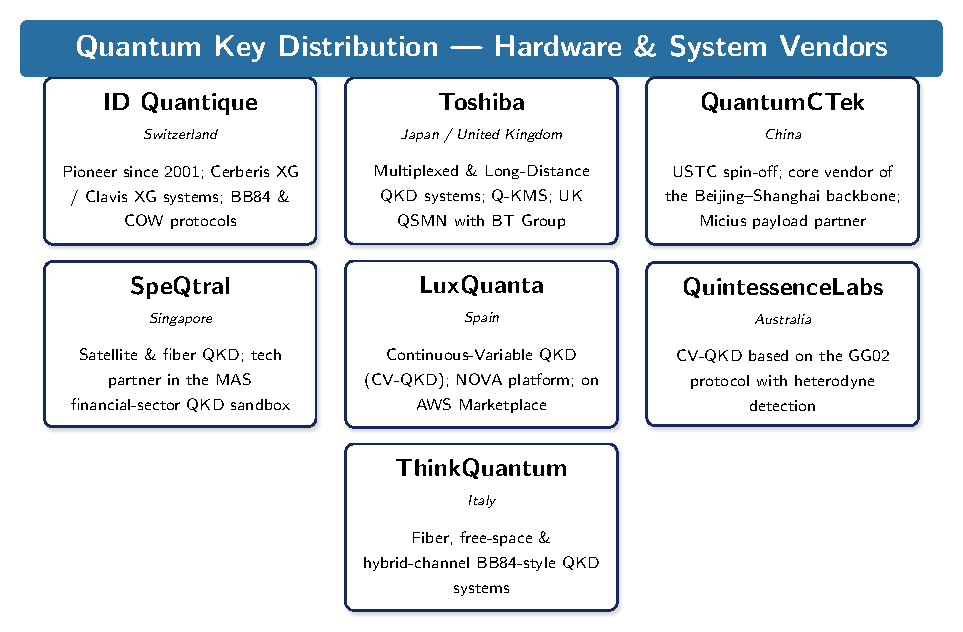
\includegraphics[width=0.98\linewidth]{figs/fig_qkd_vendors.pdf}
% TODO: لوگو، در صورت تمایل به افزودن لوگوی رسمی شرکت‌ها، فایل‌های تصویر را در
% figs/logos/ قرار دهید (راهنما در figs/logos/README.txt) و مثلاً به‌صورت زیر
% یک ردیف لوگو زیر همین شکل اضافه کنید:
% \vspace{4pt}
% \includegraphics[height=1.1cm]{figs/logos/idquantique.png}\hfill
% \includegraphics[height=1.1cm]{figs/logos/toshiba.png}\hfill
% \includegraphics[height=1.1cm]{figs/logos/quantumctek.png}
\caption{تولیدکنندگان اصلی سامانه‌های سخت‌افزاری \lr{QKD} به‌همراه کشور مبدأ و تخصص فنی \Cite{arxiv2507maturity,idq2025cerberis,toshiba2026qkd,mas2026sandbox,arxiv2307feasibility}}
\label{fig:qkdvendors}
\end{figure}

علاوه‌بر تولیدکنندگان تجاری، فعالیت گسترده در حوزهٔ ثبت اختراع نیز نشان‌دهندهٔ بلوغ روزافزون این صنعت است؛ برای نمونه، یک اختراع ثبت‌شدهٔ چینی با عنوان «روش و دستگاه ارتقای امنیت شبکهٔ توزیع کلید کوانتومی» \Cite{uspto2022patent} مستقیماً به چالش امنیت گرهٔ مورد اعتماد (بخش \ref{sec:trustednode}) می‌پردازد، نشانه‌ای از اینکه این آسیب‌پذیری، هم‌اکنون کانون توجه تحقیق و توسعهٔ صنعتی است.

%=====================================================================
